\documentclass[pageno]{jpaper}

%replace XXX with the submission number you are given from the ASPLOS submission site.
\newcommand{\asplossubmissionnumber}{XXX}

\usepackage[normalem]{ulem}

\begin{document}

\title{
Instructions for Submission to ASPLOS 2023}

\date{}
\maketitle

\thispagestyle{empty}

\begin{abstract}

This document is intended to serve as a sample for submissions to the
28th International Conference on Architectural Support for Programming
Languages and Operating Systems (ASPLOS), 2023.  It provides
guidelines that authors should follow when submitting papers to the
conference. 

\end{abstract}

\section{Introduction}

This document provides instructions for submitting papers to the 28th
International Conference on Architectural Support for Programming
Languages and Operating Systems (ASPLOS), 2023.  In an effort to
respect the efforts of reviewers and in the interest of fairness to
all prospective authors, we request that all submissions to ASPLOS
2023 follow the formatting and submission rules detailed below.
Submissions that violate these instructions may not be reviewed, at the
discretion of the program co-chairs.

The submission instructions are also available in
\href{https://asplos-conference.org/submissions/}{this website},
including a link to the paper submission site. The website contains
sample PDF files for the paper
and
extended abstract. The
sample files are formatted using the ASPLOS'23 submission format and
contain the submission and formatting guidelines. The website also
includes an archive file
with \LaTeX~templates for both papers and extended abstracts.

All questions regarding paper formatting and submission should be directed
to the program co-chairs.


\paragraph{Important highlights:}
\begin{itemize}
\item Papers should contain a
maximum of 13 pages of single-spaced two-column text but not including
references.
\item Papers should contain a maximum of {\bf 8800 words} not including references.
\item All submitted papers must be accompanied by an extended
  abstract, in a separate file with a maximum of 
2 pages of single-spaced two-column text, not counting references.
\item Papers and extended abstracts must be submitted in printable PDF format.
\item Text must be in a minimum 10pt ({\bf not} 9pt) font.
\item No page limit for references for papers and the extended abstracts.
\item Each reference must specify {\em all} authors (no {\em et al.}).
\item Proceedings will appear in the ACM digital library up to two weeks
before the conference.
\end{itemize}

\section{Paper and Abstract Preparation Instructions}

\subsection{Paper Formatting}

Papers must be submitted in printable PDF format and should contain a
maximum of {\bf 13 pages} of single-spaced two-column text, not counting
references. Papers should contain less than {\bf 8800 words} (not including references). The paper may include any number of pages for
references, but see below for more instructions. If you are using
\LaTeX~\cite{lamport94} to typeset your paper, then we suggest that
you use the template that we provide online.
If you use a different
software package to typeset your paper, then please adhere to the
guidelines given in Table~\ref{table:formatting}.

\begin{table}[h!]
  \centering
  \begin{tabular}{|l|l|}
    \hline
    \textbf{Field} & \textbf{Value}\\
    \hline
    \hline
    File format & PDF \\
    \hline
    Page limit & 13 pages, {\bf not }\\
               & {\bf including references}\\
    \hline
    Paper size & US Letter 8.5in $\times$ 11in\\
    \hline
    Top margin & 1in\\
    \hline
    Bottom margin & 1in\\
    \hline
    Left margin & 1in\\
    \hline
    Right margin & 1in\\
    \hline
    Body & 2-column, single-spaced\\
    \hline
    Word count & 8800 words\\
    \hline    
    Separation b/t columns & 0.25in\\
    \hline
    Body font & 10pt\\
    \hline
    Abstract font & 10pt, italicized\\
    \hline
    Section heading font & 12pt, bold\\
    \hline
    Subsection heading font & 10pt, bold\\
    \hline
    Caption font & 9pt, bold\\
    \hline
    Figure \& Table width & Min.~of column width or  \\
    & no more than 2    \\
    &  horizontally across the \\
    & page \\
    \hline
    References & 8pt, no page limit, list \\
               & all authors' names\\
    \hline
  \end{tabular}
  \caption{Formatting guidelines for submission. }
  \label{table:formatting}
\end{table}

\textbf{Please ensure that you include page numbers with your
submission}. This makes it easier for the reviewers to refer to different
parts of your paper when they provide comments.

Please ensure that your submission has a banner at the top of the title
page, as shown in
this
sample paper, which contains the submission number and the notice of
confidentiality.  If using the template, just replace XXX with your
submission number.

\subsection{Extended Abstract Formatting}

The extended abstracts must be submitted in printable PDF format and should contain a
{\bf maximum of 2 pages} of single-spaced two-column text, {\bf not
  counting references}.  You may include any number of pages for
references, but see below for more instructions. The extended
abstracts should use the same formatting as the papers. If you are using
\LaTeX~\cite{lamport94} to typeset your extended abstract, then we suggest that
you use
our
  template that also describes what information to include in your
extended abstract. 

The extended abstract and the paper must be independent (standalone) documents that a reviewer can read separately, as some rejection decisions may be made based only on extended abstracts. The extended abstract can refer to figures and sections in the main paper.

You can check the extended abstracts of papers published at ASPLOS 2021 
\href{https://asplos-conference.org/2021/index.html%3Fp=2181.html}
{here}.

\subsection{Content}

\noindent\textbf{Anonymity.}  Reviewing will be \textbf{double blind};
therefore, please \textbf{do not include any author names on any submitted
documents} except in the space provided on the submission form.  

Pay attention not to reveal the author or affiliation information through
side channels:

\begin{itemize}
\item The metadata included in the PDF should not give away such
information. 

\item If you are improving upon your prior work, refer to your prior
work in the third person and include a full citation for the work in the
bibliography.  For example, if you are building on {\em your own} prior
work in the papers \cite{nicepaper1,nicepaper2,nicepaper3}, you would say
something like: "Prior work
\cite{nicepaper1,nicepaper2,nicepaper3} did X, Y, and Z, this paper
additionally does W, and is therefore much better."  Do NOT omit or
anonymize references for blind review, unless
your own prior work appeared in IEEE CAL or workshops without archived
proceedings, as discussed later in this document.

\item If your system is already released to the public, please rename your system in your submission.

\item You should avoid revealing affiliation (e.g., by identifying your company’s name) in your paper. Instead, please use a generic name, like “a cloud service provider X”.  
If concealing system name or affiliation would make your paper difficult to understand, contact the program chairs to discuss exceptions to this policy.
\end{itemize}

(For more frequently-asked questions about double-blind reviewing, please 
consult this 
\href{https://pldi20.sigplan.org/track/pldi-2020-papers#FAQ-on-Double-Blind-Reviewing}
{FAQ from PLDI 2020}.)

\textbf{Violating the above anonymity requirement will be rejected without review}. If you have any concerns, please contact the program chairs before your paper submission.

\noindent\textbf{Figures and Tables.} Ensure that the figures and tables
are legible. 
Reviewers may print the papers in gray-scale. Therefore, if you use
colors for your figures, ensure that the different colors are highly
distinguishable in gray-scale. Figures and Tables must be no smaller than a column width.  There may be no more than two tables or figures horizontally across the page.

\noindent\textbf{References.}  There is no length limit for references.
Each reference must explicitly list all authors of the paper.
Knowing all authors of related
work will help find the best reviewers. Since there is no length limit
for the number of pages used for references, there is no need to save space
here.

\begin{figure*}[t!bhp]%
    \centering
    \subfloat[]{{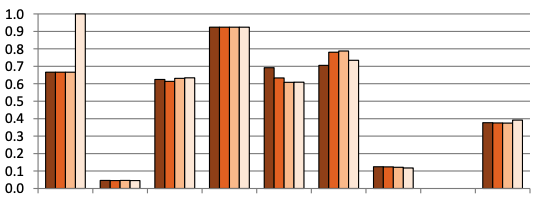
\includegraphics[width=1.0\columnwidth]{Figure1.png} }}
    \subfloat[]{{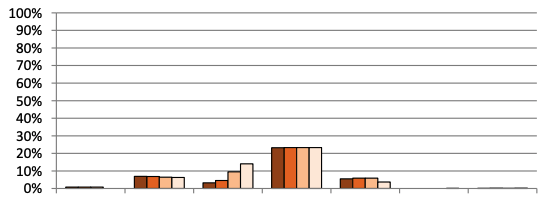
\includegraphics[width=1.0\columnwidth]{Figure2.png} }}

    \caption{Two figures side by side spanning both columns. This figure sizing is acceptable.}%
    \label{fig:twosidebyside-ok}%

\end{figure*}

\subsection{New Figure Formatting Requirements}

This section provides examples of acceptable and unacceptable figure formatting for ASPLOS 23. Figures must be a minimum of a column width. Two side-by-side figures are permitted if they span 2 columns as shown in Figure~\ref{fig:twosidebyside-ok}. Squeezing two figures into one column is not acceptable (Figure~\ref{fig:twosidebyside-no}) unless they are stacked vertically (Figure~\ref{fig:twostacked}). Three figures across are not acceptable (Figure~\ref{fig:threesidebyside}). 



\begin{figure}[t]%
    \centering
    \subfloat[]{{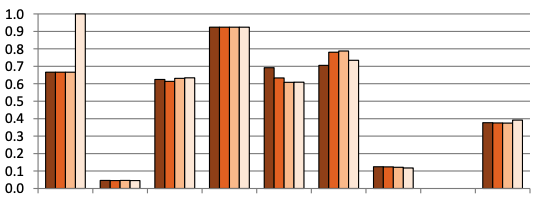
\includegraphics[width=0.49\columnwidth]{Figure1.png} }}
    \subfloat[]{{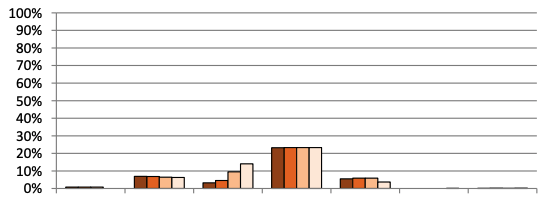
\includegraphics[width=0.49\columnwidth]{Figure2.png} }}

    \caption{Two figures each one half column width. This figure sizing is NOT acceptable.}%
    \label{fig:twosidebyside-no}%

\end{figure}

\begin{figure}[t]%
    \centering
    \subfloat[]{{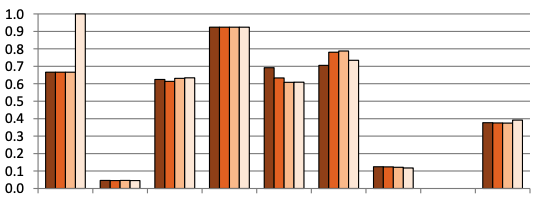
\includegraphics[width=0.99\columnwidth]{Figure1.png} }} \\
    \subfloat[]{{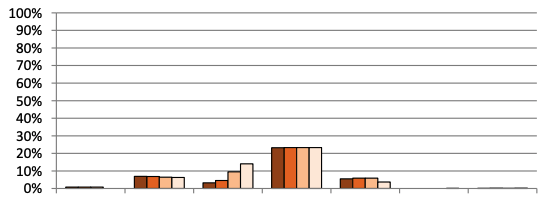
\includegraphics[width=0.99\columnwidth]{Figure2.png} }}

    \caption{Two figures stacked vertically. This figure sizing is acceptable.}%
    \label{fig:twostacked}%

\end{figure}

\begin{figure*}[t]%
    \centering
    \subfloat[]{{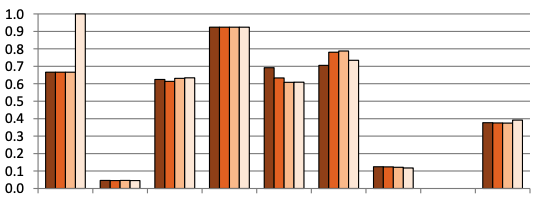
\includegraphics[width=0.67\columnwidth]{Figure1.png} }}
    \subfloat[]{{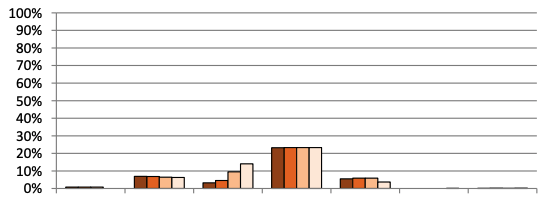
\includegraphics[width=0.67\columnwidth]{Figure2.png} }}
\subfloat[]{{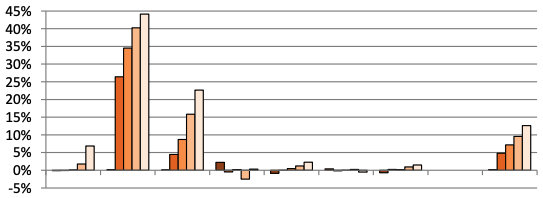
\includegraphics[width=0.67\columnwidth]{Figure3.png} }}
    \caption{Three figures spanning two columns. This figure sizing is NOT acceptable.}%
    \label{fig:threesidebyside}%

\end{figure*}

\section{Paper and Abstract Submission Instructions}

\subsection{Declaring Authors}

Declare all the authors of the paper up front. Addition/removal of authors
once the paper is accepted will have to be approved by the program co-chairs,
since it potentially undermines the goal of eliminating conflicts for
reviewer assignment.

\subsection{Areas and Topics}

ASPLOS emphasizes multidisciplinary research. Submissions should ideally
emphasize synergy of two or more ASPLOS areas: architecture, programming
languages, operating systems, and related areas (broadly
interpreted). Authors should indicate these areas on the submission form.

Authors should also indicate \textbf{at most 3}
topics covered by the paper on the submission form 
for optimal reviewer match. If more than 3 topics are selected, some topics
will be randomly dropped by program chairs.

If
you are unsure whether your paper falls within the scope of ASPLOS, please
check with the program co-chair -- ASPLOS is a broad, multidisciplinary
conference and encourages new topics.

\subsection{Declaring Conflicts of Interest}

Authors must register all their conflicts on the paper submission site.
Conflicts are needed to ensure appropriate assignment of reviewers.
If a paper is found to have an undeclared conflict that causes
a problem OR if a paper is found to declare false conflicts in order to
abuse or ``game'' the review system, the paper may be rejected.

Please declare a conflict of interest (COI) with the following people
for any author of your paper:

\begin{enumerate}
\item Your Ph.D. advisor(s), post-doctoral advisor(s), Ph.D. students,
      and post-doctoral advisees, forever.
\item Family relations by blood or marriage and close personal friends, forever (if they might be potential reviewers).
\item People with whom you have collaborated in the last four years, including
\begin{itemize}
\item co-authors of accepted/rejected/pending papers.
\item co-PIs on accepted/rejected/pending grant proposals.
\end{itemize}
\item People (including students) who shared your primary institution(s) in the
last four years.
\end{enumerate}

You need not and should not declare a COI for the following cases:

\begin{itemize}
\item ``Service'' collaborations such as co-authoring a report for a professional
organization or an open-source community, serving on a program committee, or co-presenting
tutorials, do not themselves create a conflict of interest.

\item Co-authoring a paper that is a compendium of various projects without
direct collaboration among the projects does not constitute a
conflict among the authors of the different projects.

\item Internships constitute a conflict of interest during the period of employment of the intern, but not thereafter, unless some other provision applies (e.g., coauthorship or ongoing research collaboration after the internship).

\item You \textbf{must not} declare a COI with a reviewer just because that reviewer works on topics similar to or related to those in your paper. 

\end{itemize}

Please declare all your conflicts, not just restricted to the PC and ERC, as we may occasionally ask for reviews from people outside the PC and the ERC. 

When in doubt, contact the program chairs.

\subsection{Concurrent Submissions and Workshops}

By submitting a manuscript to ASPLOS'23, the authors guarantee that the
manuscript has not been previously published or accepted for publication in
a substantially similar form in any conference, journal, or workshop. The
only exceptions are (1) workshops without archived proceedings such as in
the ACM digital library (or where the authors chose not to have their paper
appear in the archived proceedings), or (2) venues, such as IEEE CAL, where
there is an explicit policy that such publication does not preclude longer
conference submissions. These are not considered prior publications. 
Technical reports and papers posted on public social media sites, Web pages,
or online repositories, such as arxiv.org, are not considered prior
publications either. In these cases, the submitted manuscript may
ignore the posted work to preserve author anonymity. 
The authors also guarantee that no paper that contains
significant overlap with the contributions of the submitted paper will be
under review for any other conference, journal, or workshop during the
ASPLOS'23 review period. Violation of any of these conditions will lead to
rejection. As always, if you are in doubt, it is best to contact the
program co-chairs.  Finally, we also note that the ACM Plagiarism Policy
(http://www.acm.org/publications/policies/plagiarism\_policy) covers a range
of ethical issues concerning the misrepresentation of other works or one's
own work.

\subsection{Ethical Obligations}
\begin{itemize}
\item Authors are not allowed to contact reviewers or PC members to encourage or solicit them to bid on any paper.
\item Authors are not allowed to attempt to sway a reviewer to review any paper positively or negatively.
\item Authors are not allowed to contact reviewers or PC members requesting any type of information about the reviewing process, either in general or specifically about submitted papers.
\item Authors are not allowed to contact reviewers or PC members to ask about the outcomes of any papers.
\item Authors must also abide by the
  \href{https://www.acm.org/code-of-ethics}{ACM ethics
    policy}. Violation of the ACM ethics policy may result in
  rejection of the submission and possible action by the ACM.
 \item Authors are not allowed to advertise their submissions or related technical reports and postings (e.g., to arxiv.org or online repositories) on social media or community blogs and webpages during the period starting two weeks before the submission deadline and ending when the ASPLOS’23 acceptance results are public.
\end{itemize}

\section{Early Access in the Digital Library}

The ASPLOS'23 proceedings will be freely available via the ACM Digital
Library for up to two weeks before the
conference. Authors must consider any implications of this early
disclosure of their work {\em before} submitting their papers.



\section{Acknowledgements}

This document is modified from the ASPLOS'21 and ASPLOS/22 submission guides, thank
you Emery Berger, Christos Kozyrakis, Shan Lu and Thomas Wenisch!

\bibliographystyle{plain}
\bibliography{references}


\end{document}

